\section{Sorting}

\subsection{Bubble Sort}

입력 배열을 순회하며 두 요소를 선택한 뒤, 정렬되어 있다면 그대로 두고 아니라면 swap하며 정렬.

\begin{verbatim}
def bubble_sort(A: list[int]):
  for i in range(len(A) - 1, 0, -1):
    for j in range(i):
      if A[j] > A[j + 1]:
        A[j], A[j + 1] = A[j + 1], A[j]
\end{verbatim}

요소의 입력 순서대로 뒤쪽에 있는 요소와 앞쪽에 있는 요소를 비교해 swap하므로 stable하다. 단, L4에서 크거나 같음(>=) 비교를 하면 값이 같은 요소도 swap하게 되므로 unstable해진다.

\subsection{Selection Sort}

입력 배열을 순회하며 커서 뒤의 최소값과 커서의 값(정렬되지 않은 맨 앞쪽 값)을 swap하며 정렬.

\begin{verbatim}
def selection_sort(A: list[int]):
  for i in range(len(A) - 1):
    min_idx = i
      for j in range(i + 1, len(A)):
        if A[j] < A[min_idx]:
          min_idx = j
      A[i], A[min_idx] = A[min_idx], A[i]
\end{verbatim}

커서 값과 최소값을 swap하는 순서가 기존 순서와 상관없이 일으나므로 stable하지 않다. 단, 값을 swap하지 않고 insert하도록 구현하면 stable해진다.

\begin{verbatim}
def stable_selection_sort(A: list[int]):
  n = len(A)
  for i in range(n-1):
    min_idx = i
    for j in range(i+1, n):
      if A[min_idx] > A[j]:
        min_idx = j
    key = A[min_idx]
    while min_idx > i:
      A[min_idx] = A[min_idx-1]
      min_idx -= 1
    A[i] = key
\end{verbatim}

\subsection{Insertion Sort}

입력이 이미 정렬되어 있으면 모든 원소가 제자리에 있게 되므로 최선의 경우 $O(n)$. 따라서 원소 개수가 적거나 거의 정렬되어 있을 때 좋은 성능을 보인다.

\begin{verbatim}
def insertion_sort(A: list[int]):
  for i in range(1, len(A)):
    k = A[i]
    j = i - 1
    while j >= 0 and k < A[j]:
      A[j + 1] = A[j]
      j -= 1
    A[j + 1] = k
\end{verbatim}

입력 요소의 순서를 유지한 상태에서 자신보다 큰 요소들을 한 자리씩 뒤로 밀고 그 앞에 insert하는 방식이므로 stable하다. 단, 4번째 줄에서 크거나 같음(>=) 비교를 하면 값이 같은 요소도 뒤로 밀게 되므로 unstable해진다.

\subsection{Shell Sort}

삽입 정렬을 응용한 알고리즘. 대략 정렬을 해놓고 삽입 정렬을 한다.

\begin{enumerate}
  \item 우선 gap에 따라 숫자를 여러 그룹으로 나누고, 각 그룹 내에서 삽입 정렬을 한다.
  \item 이어서 gap을 줄이며 같은 방식으로 정렬을 수행한다.
  \item 마지막에는 반드시 gap을 1로 놓고 정렬한다. 다른 그룹에 속해 서로 비교되지 않은 숫자가 있을 수 있기 때문. 이는 삽입 정렬 그 자체다.
\end{enumerate}

\begin{verbatim}
def shell_sort(A: list[int]):
  h = len(A) // 2
  while h > 0:
    for i in range(h, len(A)):
      k = A[i]
      j = i
      while j >= h and k < A[j - h]:
        A[j] = A[j - h]
        j = j - h
      A[j] = k
    h = h // 2
\end{verbatim}

시간복잡도는 $O(n^2)$. gap에 따라 성능이 좌우된다. 가장 좋은 성능의 gap으로 알려진 히바드 간격 $2^k - 1$은 $O(n^{1.5})$. 많은 실험으로 통해 $O(n^{1.25})$로 알려짐. 입력 크기가 매우 크지 않은 경우 좋은 성능을 보인다.

\subsection{Heap Sort}

힙을 이용하는 정렬. 최대 힙은 항상 상위 노드의 값이 하위 노드의 값보다 큰 완전 이진트리. 과정을 $(n - 1)$번 반복하므로 총 시간 복잡도는 $O(n) + (n - 1) * O(\log n) = O(n \log n)$.

\begin{enumerate}
  \item 리스트를 최대 힙으로 만든다. 이때 순서는 BFS. heapify로 $O(n)$ 시간이 든다.
  \item 루트와 마지막 노드를 교환한다. 이제 마지막 노드는 정렬된 상태이므로, 힙 트리에서 마지막 노드를 제거한다.
  \item 깨진 힙을 다운 힙으로 재구조화한다. 다운 힙 시에는 대상 노드와 그 하위 두 노드 중 더 큰 것과 교환한다. 이때 heapify에 드는 시간은 트리의 높이인 $O(\log n)$.
  \item 2, 3을 반복한다.
\end{enumerate}

힙을 배열에 저장할 때는 \texttt{A[0]}를 비워두고, \texttt{A[1]}부터 \texttt{A[n]}까지 힙 노드들을 트리의 층별로 저장한다. 가령 \texttt{A[1]}에 루트 노드를 저장했다면, \texttt{A[2]}에는 왼쪽 하위 노드를, \texttt{A[3]}에는 오른쪽 하위 노드를 저장한다. 완전 이진 트리이기 때문에 아래의 공식이 유효하다.

\begin{itemize}
  \item \texttt{A[i]}의 상위 노드: \texttt{A[i / 2]}
  \item \texttt{A[i]}의 왼쪽 하위 노드: \texttt{A[2 * i]}
  \item \texttt{A[i]}의 오른쪽 하위 노드: \texttt{A[2 * i + 1]}
\end{itemize}

최대 힙으로 구현된 힙 정렬은 루트 노드와 마지막 노드를 교환하는 과정에서 앞에 있는 중복 요소가 그 뒤에 배치된다. 따라서 unstable하다.

\subsection{Radix Sort}

지금까지 다룬 정렬 알고리즘은은 숫자와 숫자를 비교를 하는 비교 정렬(comparison sort)이었음. 반면 기수 정렬은 숫자를 한 자리씩 부분적으로 비교함.

기수 정렬은 비교 정렬과 달리 숫자를 부분적으로 비교한다. 1의 자리부터 $k$번째 자리로 진행하는 LSD 기수 정렬을 살펴보자. $k$자리 부터 1의 자리로 진행하는 방식은 MSD라고 한다.

\begin{enumerate}
  \item 우선 각 숫자의 1의 자리를 비교해 정렬한다.
  \item 다음엔 10의 자리를 비교해 정렬한다. 중복되는 숫자가 있는 경우 전 단계의 순서를 그대로 따라야 한다. 이것을 안정성이라고 한다.
  \item 마찬가지로 100의 자리, 1000의 자리를 비교해 안정 정렬한다.
\end{enumerate}

기수 정렬의 시간복잡도는 $O(k(n + r))$. 이때 자리수 $k$나 상수 $r$이 입력 크기 $n$보다 작으면 $O(n)$이다. 이는 각 자리에 들어갈 숫자가 전제되기 때문에 가능한 것. 숫자를 그대로 인덱스로 쓸 수 있다. 문자열이라도 어떤 문자만 사용할지 전제하면 가능하다. 이렇게 한정된 조건에서만 사용할 수 있기 때문에 정렬 문제의 하한이 $O(n)$이라고 할 수는 없음.

\subsubsection{비교 정렬의 하한}

비교 정렬을 이용하는 경우 정렬 문제의 하한을 알아보자. 문제의 하한이란 그 문제를 풀기 위한 어떠한 알고리즘이라도 해를 구하려면 적어도 하한의 시간복잡도만큼 시간이 걸린다는 뜻. 3개의 숫자를 정렬할 때 결정 트리는 리프 노드의 수가 $3!$개인 이진트리. 여기에는 정렬에 불필요한 내부 노드가 없다. 따라서 어느 경우라도 서로 다른 3개의 숫자를 정렬하려면 적어도 3번의 비교가 필요하다.

n개의 서로 다른 숫자를 정렬하는 결정 트리의 높이를 계산하려면 이진트리의 속성을 이용한다: $k$개의 리프 노드가 있는 이진 트리의 높이는 $\log k$보다 크다. 따라서 $n!$개의 리프를 가진 결정 트리의 높이는 $\log(n!)$보다 크다. 이때 $\log(n!) = O(n \log n)$이므로, 비교 정렬의 하한은 $O(n \log n)$.

\subsubsection{안정성}

입력에 중복된 숫자가 있을 때 정렬 후에도 중복된 숫자의 순서가 입력 순서와 동일한 것을 말한다. 가령 $3a, 2b, 4c, 3d, 1e$가 입력됐을 때 안정한 정렬(stable sort)의 결과는 $1e, 2b, 3a, 3d, 4c$가 되어야 한다. 기수 정렬이 이를 지키지 않으면 전 단계의 정렬이 무효해진다.

안정 정렬은 원래 원소들 간의 상대적인 순서를 유지하면서 정렬해야 할 때, 정렬 기준이 여러 개일 때 필요하다. 버블 정렬, 삽입 정렬, 병합 정렬은 안정적이다. 선택 정렬, 쉘 정렬, 퀵 정렬, 힙 정렬은 불안정하다. 병합 정렬의 경우 분할된 부분 리스트가 기존 순서를 유지하고 있고, 이를 병합할 때도 순서를 유지한다. 반면 퀵 정렬의 경우 pivot을 기준으로 원소를 왼쪽, 오른쪽 부분으로 재배치하고 정렬을 하기 때문에 기존 순서를 유지할 수 없다.

\subsection{External Sort}

\textbf{내부 정렬(Internal sort)}: 입력의 크기가 메인 메모리의 공간보다 크지 않은 경우에 수행되는 정렬. 지금까지 다룬 정렬 알고리즘은 모두 내부 정렬.

\noindent \textbf{외부정렬(External sort)}: 입력의 크기가 메인 메모리보다 큰 경우. 보조 기억 장치에 있는 입력을 여러 번에 나누어 메인 메모리에 읽어 들인 후 정렬하여 보조 기억 장치에 다시 저장하는 과정을 반복한다.

\begin{enumerate}
  \item HDD A에서 순차적으로 데이터를 읽어 메인 메모리에 로드한다.
  \item 메인 메모리는 데이터가 로드될 때마다 내부 정렬을 하고 HDD B에 저장한다.
  \item HDD B에 저장된 데이터 블록 2개를 선택하고 각 블록의 데이터를 부분적으로 메인 메모리에 로드해 병합한다.
  \item 메인 메모리는 두 블록을 번갈아가며 순차적으로 HDD A에 저장한다.
\end{enumerate}

외부정렬은 전체 데이터를 몇 번 처리하는지에 따라 시간복잡도를 측정. 전체 데이터를 읽고 쓰는 것을 패스라고 한다. 입력 크기가 $N$이고 메인 메모리 크기가 $M$이라면 시간복잡도는 $O(\log(N / M))$.

\section{NP-Complete}

\begin{figure}[h]
  \centering
  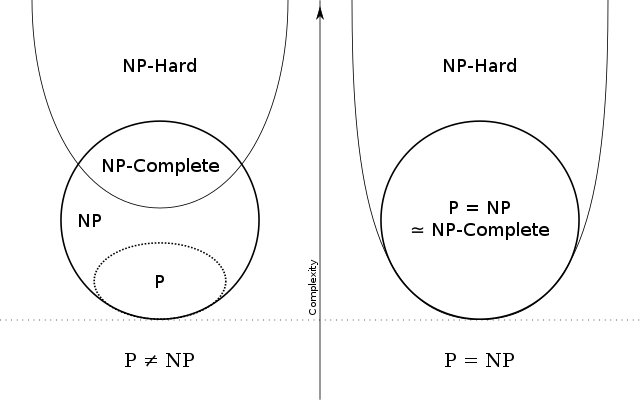
\includegraphics[width=\columnwidth]{p-np-diagram.png}
\end{figure}

문제는 크게 두 개 집합으로 분류할 수 있다.

\begin{itemize}
  \item 다항식 시간복잡도 알고리즘으로 해결되는 문제 집합.
    \begin{itemize}
      \item \textbf{P}: 다항식 시간 내에 결정론적으로 해를 찾을 수 있는 문제의 집합. 즉, 시간복잡도가 $O(n^k)$에 포함되는 경우.
      \item \textbf{NP}: 다항식 시간 내에 비결정론적으로 해결되는 문제의 집합. 즉, NP 문제는 비결정 튜링 머신으로 다항식 시간에 해결 가능하다. 문제의 조건을 만족하는 해가 존재하는지 판단하는 결정 문제를 다항식 시간에 확인할 수 있는 경우에도 NP 문제.
    \end{itemize}
  \item 다항식보다 큰 시간복잡도 알고리즘으로 해결되는 문제 집합.
    \begin{itemize}
      \item \textbf{NP-Complete}: NP 문제 중 지수 시간의 시간복잡도를 가진 알고리즘으로 해결되는 문제 집합.
      \item \textbf{NP-Hard}: 어떤 NP 문제보다도 해결하기 어려운 문제.
    \end{itemize}
\end{itemize}

P 문제 집합이 NP 문제 집합에 속하는 이유: P 문제를 해결하는데 다항식 시간이 걸리므로, 이를 NP 알고리즘이 문제의 해를 다항식 시간에 확인하는 것과 대응시킬 수 있기 때문.

\subsection{Turing Machine}

\begin{figure}[h]
  \centering
  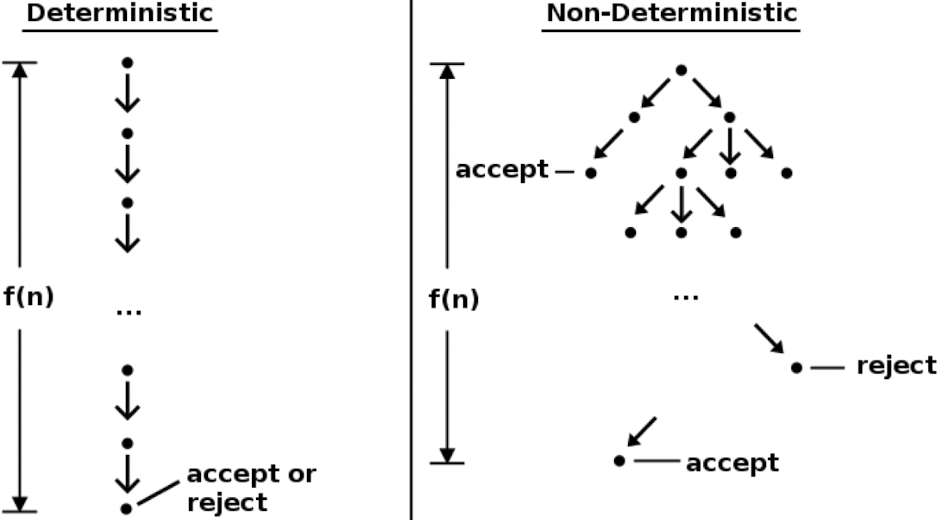
\includegraphics[width=\columnwidth]{non-deterministic-turing-machine.png}
\end{figure}

튜링 머신은 입력에 대해 출력을 내는 가상의 컴퓨터. 비결정 튜링 머신은 특정 상태에서 움직일 수 있는 다음 상태의 개수가 하나로 정해져 있지 않은 튜링 머신을 말한다. 일정 시간 안에 해를 찾을 수도, 못 찾을 수도 있다. NP 문제가 비결정 튜링 머신으로 해결된다는 건 비결정 튜링 머신이 아주 운이 좋은 경우 다항식 시간에 해결할 수 있다는 것. 유한상태기계는 입력에 따라 상태가 변화하는 튜링 머신.

\subsection{Reduction}

NP 완전 문제 A를 해결하기 위해 문제 B를 해결하는 알고리즘을 이용하는 것. 이렇게 하면 밖에서는 A 문제를 푼 것으로 보인다.

가령 문제 A는 원소의 합이 $K$가 되게 만드는 부분 집합을 찾는 `subset sum' 문제. $O(2^n)$ 시간이 걸리는 NP 완전 문제임. 문제 B는 두 부분 집합 $X$, $Y$의 합을 같게 만드는 `partition' 문제.

\begin{figure}[h]
  \centering
  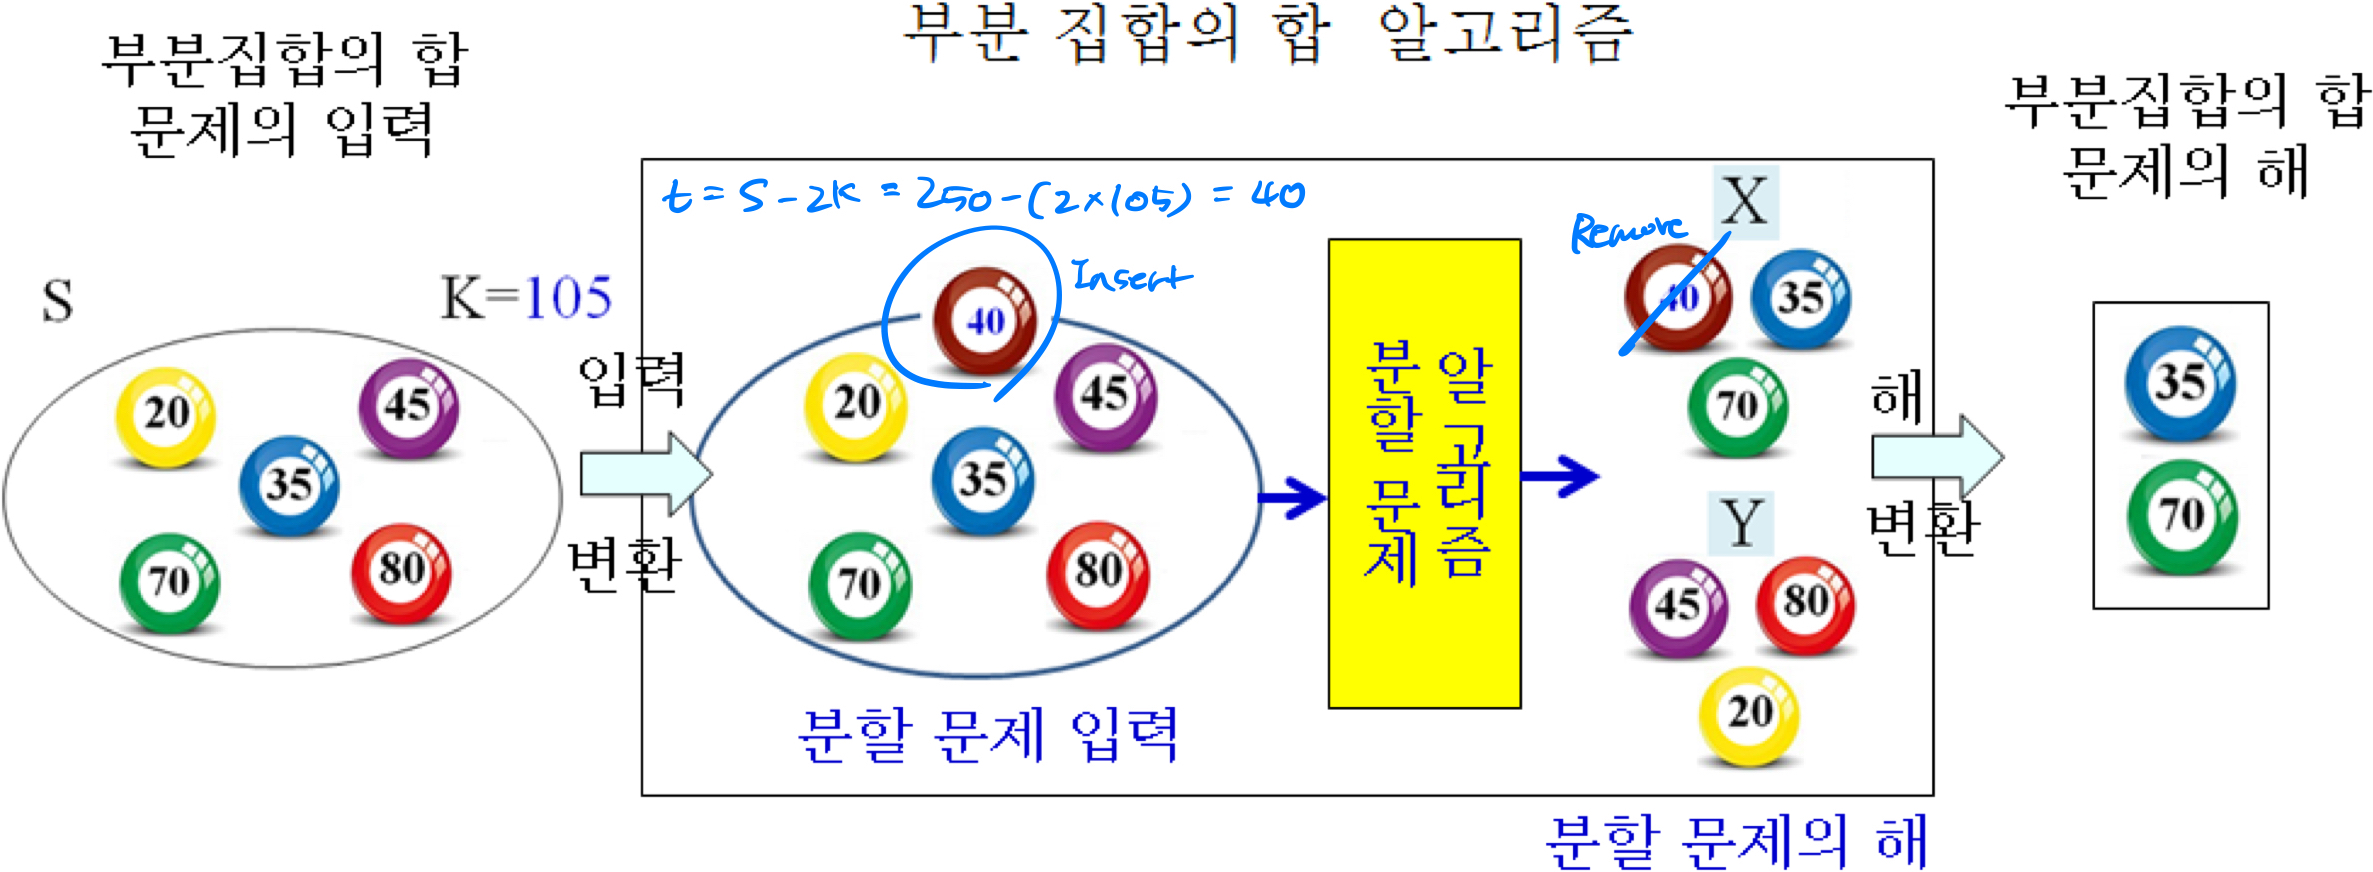
\includegraphics[width=\columnwidth]{np-c-set-example.jpeg}
\end{figure}

변환의 시간복잡도는 입력 변환 시간, 문제 B 알고리즘의 수행 시간, 출력 변환 시간의 총합.

입력과 출력의 변환은 다항식 시간에 가능하다. 이때 문제 A는 문제 B로 reducible하다. 양쪽으로 reducible하다면 transitive한 관계. 추이 관계로 NP-C 문제들이 서로 얽혀 있어서 어느 하나의 문제에 대해 다항식 시간에 해를 구할 수 있다면 다른 모든 NP-C 문제도 다항식 시간에 해를 구할 수 있다.

\section{Approximation}

NP-C 문제는 실세계에서 광범위하게 활용되지만, 다항식 시간에 해결할 방법이 발견되지 않음. 근사 알고리즘은 최적해 찾는 걸 포기하고 다항식 시간에 모든 입력에 대한 해를 찾음. 단, worst case에서 근사해가 최적해에 얼마나 가까운지 나타내는 근사 비율을 함께 제시해야 함.

\subsection{Traveling Salesman Problem}

임의의 도시에서 출발해 다른 모든 도시를 한 번씩만 방문하고 출발지로 돌아오는 경로의 길이를 최소화하는 문제.

\begin{enumerate}
  \item MST를 만든다.
  \item 한 도시에서 출발해 모든 도시를 방문하고 돌아오는 순서를 구한다.
  \item 앞서 구한 순서를 따라 방문하되, 중복 방문하는 도시를 순서에서 제거한다. (단, 마지막 도시는 출발 도시와 같으므로 제거하지 않는다.)
\end{enumerate}

이때 근사 비율은 MST 선분의 가중치 합($M$)을 간접적인 최적해로 사용해 구한다. 실제 최적해 값도 $M$보다는 같거나 클 것이기 때문이다. 앞의 알고리즘에 따르면 근사 비율은 $2M / M = 2$. 즉, 근사해의 값이 최적해의 2배를 넘지 않는다.

\subsection{Vertex Cover}

그래프에서 각 선분의 양 끝점 중 적어도 하나의 끝점을 포함하는 점들의 집합 중 최소 크기의 집합을 찾는 문제. CCTV를 설치한다고 하면 모든 간선을 감시할 수 있는 위치를 찾는 것.

따라서 사실 정점이 아니라 간선을 선택하는 것. 간선 하나를 선택하면 정점 두 개를 선택하는 셈. 임의의 선분을 선택하면 주변의 커버된 선분은 이후 선택하지 않는다. 이렇게 선택된 선분 집합을 극대 매칭이라고 함.

\begin{figure}[h]
  \centering
  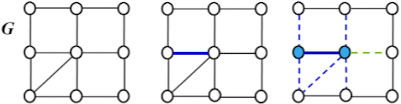
\includegraphics[width=\columnwidth]{vertex-cover-appx.png}
\end{figure}

극대 매칭을 찾기 위해 하나의 간선을 선택할 때 $O(n)$, 그래프의 간선 수가 $m$이라면 각 선분에 대해 $O(n)$ 시간. 따라서 $O(mn)$.

근사 비율은 극대 매칭을 간접적인 최적해로 사용해 구한다. 어떠한 정점 커버라도 극대 매칭에 있는 선분을 커버해야 하기 때문. 근사해의 값은 극대 매칭 선분 수의 2배. 따라서 근사 비율은 극대 매칭의 각 선분의 양 끝점의 수를 극대 매칭의 간선 수로 나눈 2.

\subsection{Bin Packing}

$n$개의 물건과 용량이 $C$인 통이 있을 때, 모든 물건을 가장 적은 수의 통에 채우는 문제. 물건을 통에 넣으려면 통에 그 물건이 들어갈 여유가 있어야 한다. 그리디하게 근사하는 몇가지 방법이 있음.

\begin{itemize}
  \item 최초 적합: 첫 번째 통부터 차례로 살펴보며, 가장 먼저 여유가 있는 통을 선택.
  \item 다음 적합: 직전에 물건을 넣은 통에 여유가 있으면 선택.
  \item 최선 적합: 기존 통 중에서 물건이 들어가면 남는 부분이 가장 작은 통을 선택.
  \item 최악 적합: 기존 통 중에서 물건이 들어가면 남는 부분이 가장 큰 통을 선택.
\end{itemize}

다음 적합은 직전에 사용한 통만 살펴보면 되므로 $O(n)$. 이때 근사 비율은 최적해의 2배를 넘지 않는 2.

나머지 방법은 물건을 넣을 때마다 모든 통을 살펴봐야 하므로 $O(n^2)$. 2개 이상의 통이 $1 / 2$ 이하로 차 있는 경우는 없다. 따라서 2.

\subsection{Job Scheduling}

작업의 시작 시각이 아니라 수행 시간을 고려. 그리디하게 근사할 수 있음. 가장 빠르게 현재 작업을 수행할 수 있는 기계에 배정한다. $n$개의 작업에 대해 $m$개 기계의 종료 시간을 확인해야 하므로 $O(nm)$. 근사 비율은 2.

\subsection{Clustering}

K-Means와 동일한 문제. $n$개의 점에 대해 $k$개의 센터까지의 거리를 각각 계산해야 하므로 $O(k^2 n)$. 근사 비율은 2.

\section{Solution Finding}

NP-C 문제는 $n$이 너무 크지 않다면, 느리더라도 모든 경우를 다 해보고 해결할 수 있다. 미로 탐색의 경우 오른손을 짚고 가는 DFS(Depth First Search)로 해결 가능. 하지만 최단 경로가 아니다.

\subsection{Backtracking}

해를 찾는 도중에 막히면(도달한 리프 노드가 해가 아니라면) 되돌아가서 다시 해를 찾는 기법. 특정 조건을 최소화/최대화하는 조합을 찾는 최적화 문제 또는 결정 문제를 해결할 수 있다.

트리를 만들어서 모든 리프 노드에서의 값을 확인해본다. 단, 현재 알고 있는 최적의 값(최단 경로)보다 값이 더 커지는 시점에 그 하위 트리는 탐색하지 않는 pruning을 할 수 있다.

백트래킹의 시간 복잡도는 상태 공간 트리의 노드 수에 비례. 최악의 경우 모든 노드를 탐색하는 완결 탐색(exhaustive search)과 같아지므로 지수 시간이 걸린다. 평균적으로는 pruning을 하기 때문에 훨씬 효율적임.

\subsection{Branch-and-Bound}

트리의 각 노드(state)에 한정값(bound)을 부여하고, 노드의 한정값을 활용해 pruning함으로써 백트래킹보다 빠르게 해를 찾는다. 백트래킹과 다른 점은 어떤 노드의 가능성이 높을 지 예측하고, 가능성이 높은 노드부터 탐색한다는 것.한정값을 잘못 정하면 단순히 루트 노드와 가까운 노드부터 탐색하게 되므로 BFS와 같아진다. 미래를 고려해 정해야 하는데, 대충 정하면 더 나은 경로가 있음에도 선택하지 않는 문제가 생길수도. Branch-and-Bound는 깊이 우선이 아니라 최선 우선이기 때문에 `best first search'.

공짜 점심은 없다. 일반적으로 백트래킹보다 효율적이지만, 메모리 사용량이 커질수도. 백트래킹은 스택을 쓰기 때문에 트리의 깊이만큼만 메모리를 사용함. 따라서 공간복잡도가 $O(n)$. 하지만 best first search는 pruning이 잘 안 된 경우 큐 크기가 엄청 커질 수 있음. 참고로 BFS는 exhaustive함. BFS는 다음 레벨의 모든 노드를 큐에 담아야 하기 때문에 공간복잡도가 $O(n!)$.

\subsubsection{TSP}

임의의 위치 x에서의 한정값은 x까지의 길이에 x를 떠나 남은 점을 한번씩 방문하고 시작점으로 돌아오는 경로의 예측 길이.

\begin{figure}[h]
  \centering
  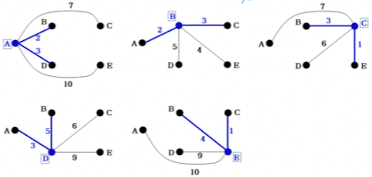
\includegraphics[width=\columnwidth]{tsp-bab.png}
\end{figure}

\begin{enumerate}
  \item 초기 한정값: 각 노드에서의 가장 작은 간선 두 개의 합을 모두 더하고 2로 나눈다.
  \item [A, B], [A, D], [A, C], [A, E] 중 하나를 선택.
  \item [A, B]를 선택: A를 거쳐온 B위치에서 한정값을 계산.
\end{enumerate}

\subsubsection{A$^\star$ Search}

branch-and-bound의 개선판. $f(n) = g(n) + h(n)$으로 노드의 가치를 표현할 수 있다.

\begin{enumerate}
  \item $f$: 시작점에서 현재 노드를 지나 도착점까지의 예상 거리.
  \item $g$: 시작점에서 현재 노드까지의 실제 거리.
  \item $h$: 현재 노드에서 도착점까지의 예상 거리.
\end{enumerate}

이때 $h$를 휴리스틱 함수라고 부르며, 길 찾기의 경우 보통 유클리드 거리나 맨해튼 거리를 사용. $h$에 따라 최적해를 만들지 못하기도 한다. $h$는 실제 도착점까지의 거리보다는 짧거나 같아야 루트와 가까운 노드가 선택될 수 있다. 이러한 함수를 admissible heuristic function이라고 부름. 최초로 도달한 리프가 최적해임을 보장할 수 있음.

그렇다고 $h$를 0으로 하면 무조건 가까운 노드가 선택되므로 BFS와 같아짐. BFS는exhaustive함. 이것도 exhaustive해서 공간복잡도가 트레이드오프이긴 한데, pruning이 잘 돼서 빠르기 때문에 사용.

\subsubsection{Genetic Algorithm}

여러 해를 임의로 생성해 초기 세대로 놓고, 루프를 통해 현재 세대의 해로부터 다음 세대의 해를 생성한다. 루프가 끝났을 때 마지막 세대에서 가장 우수한 해를 반환한다.

\begin{enumerate}
  \item 선택 연산: 여러 세대의 후보해 중에서 우수한 후보해를 선택할 때는 적합도의 확률에 따라 랜덤하게 선택한다. 이 방법을 roulette wheel이라고 한다. 적합도가 높은 후보해가 미래에도 좋을 것이라는 보장이 없기 때문에 랜덤 선택하는 것.
  \item 교차 연산: 선택 연산을 통해 얻은 우수한 후보해보다 더 우수한 후보해를 생성하는 것. 교차 연산을 수행할 후보해의 수는 0.2에서 1.0 범위의 교차율(crossover rate)를 이용해 조절한다.
  \item 돌연변이 연산: 작은 확률(mutation rate)로 후보해의 일부분을 변형. mutation rate는 보통 $(1 / \text{population size}) \sim (1 / \text{length})$ 범위. population size는 한 세대의 후보해 수, length는 후보해를 이진 표현했을 때 비트 수.
\end{enumerate}

다음 세대가 현재 세대보다 우수하지 않다면 종료한다. 최적해를 보장하지 않지만, 기존의 알고리즘으로 해결하기 어려운 경우 최적해에 가까운 해를 찾을 때 적절하다.

\subsubsection{Simulated Annealing}

이와 같은 기법을 iterative method라고 함. 솔루션을 만들어 가는게 아니라 찾아가는 것에 가까움. 어떤 시작점에서 솔루션을 조금씩 발전시켜 나간다. 따라서 시작점에 여러 후보해를 만들어 둬야 한다. 이때 후보해를 임의로 만드는데, 그래서 randomized algorithm이라고도 함.

\begin{verbatim}
set random solution s
set initial T # temperature (e.g. T = 1000)
repeat:
  for i = 1 to k: # k is number of loop at T
    selete a solution s'
      in neighbors of s randomley
    d = s' - s
    if (d < 0): s = s' # if neighbor
                       #   s' is superior to s
    else:
      q = random number in (0, 1)
      if (q < p): s = s' # p is exploration
                         #   probability
  T = A * T # multiply constant A less than 1
            #   by T to calculate a new T
until
return s
\end{verbatim}

\section{Realworld Problems}

\subsection{설탕 배달}

\begin{verbatim}
def g(a: int, b: int) -> int:
  if a == -1:
    return b
  elif b == -1:
    return a
  else:
    return min(a, b)

def f(n: int) -> int:
  d = [0] + [-1 for _ in range(n)]
  for i in range(1, len(d)):
    a, b = -1, -1
    if i >= 5 and d[i - 5] != -1:
      a = d[i - 5] + 1
    if i >= 3 and d[i - 3] != -1:
      b = d[i - 3] + 1
    d[i] = g(a, b)
  return d[n]
\end{verbatim}

